\chapter{Introduction}

A Distributed Computing System is a network of multiple computers(nodes) which collaborate in order to solve tasks. In Distributed Computing a task is divided into smaller parts and solved by different nodes. The nodes can be physically close, connected via a local network, or geographically distant, connected by a wide area network. From the outside a Distributed Computing System acts as a single computer even though it is comprised of several nodes.

\begin{figure}
	\centering
	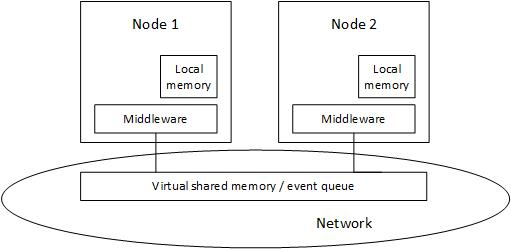
\includegraphics[width=0.8\textwidth,natwidth=610,natheight=642]{DistributedComputingSystemWith2nodes.jpg} 
	\captionsetup{format=plain,font=footnotesize,labelfont={bf,red},labelsep=quad,singlelinecheck=no}
	\caption[Distributed Computing System with 2 nodes]{
		\label{fig:distributedCoputingSystem} 
		\footnotesize{%
			A Distributed Computing System with 2 nodes.
		}
	}
\end{figure}

Figure \cref{fig:distributedCoputingSystem} illustrates the idea of a Distributed Computing System. Nodes 1 and 2 shares virtual memory and/or event queue. The Middleware handles communication between the nodes and ensures the virtual memory is consistent throughout the network. The shared virtual memory is transparent to each node. 

Distributed systems offer many benefits over centralized systems including the following:
\begin{itemize}
	\item Scalability: It is easy to add notes to the system, should the size of the system increase.
	\item Redundancy: Several nodes can provide the same service, so if a node crashes, there are many to replace it. Additionally, from a cost perspective, each node does not have to be expensive, because many smaller nodes can be used as replacement.
\end{itemize}

\section{Thesis motivation}
The following chapter describes the motivation for this thesis. First a case from Siemens Wind Power is presented, followed by the Thesis motivation.

\subsection{Siemens Wind Power case}
\label{sec:SiemensCase}
Siemens Wind Power is among the leading windmill manufacturers in the world. Siemens builds wind farms of different sizes ranging form single mills to well above one hundred windmills \cite{simensOffShoreProjects, simensOnShoreProjects}.

Today windmills in a windmill farm at Siemens are equipped with a computer for the purpose of regulating power production parameters, data collection and for communication with the rest of the system. The current setup is illustrated on \cref{fig:currentSiemensSetup}. Every windmill is connected to a Wind Power Supervisor (WPS), which is a central component that aggregates data, perform calculations, store data and handle windmill farm communication with the outside world. At Siemens up to 8 WPS's are present pr. windmill farm.

A database is deployed on every WPS, for aggregated data collected from each windmill. Every windmill has a database as well for data logging purposes. The windmills, WPS's and Park Regulator are connected with a gigabit network, which currently has plenty of extra capacity. The system handles more than 50 control points and 200 measurement points and samples these every 50 ms. The Park Regulator regulates the power production when needed. See \cref{fig:dataComputationSequence} for the regulation sequence.

\begin{figure}
	\centering
	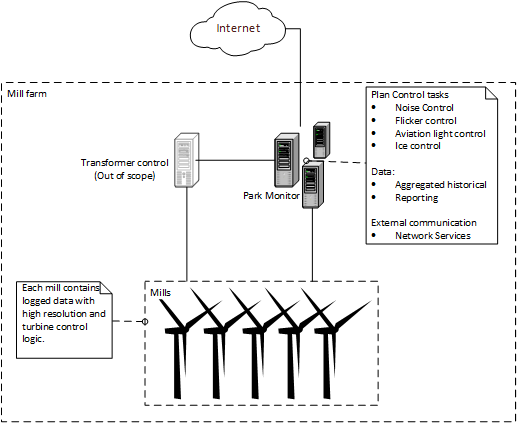
\includegraphics[width=0.7\textwidth,natwidth=610,natheight=642]{SystemOverviews.png} 
	\captionsetup{format=plain,font=footnotesize,labelfont={bf,red},labelsep=quad,singlelinecheck=no}
	\caption[Illustrates the current Siemens windmill farm setup]{
		\label{fig:currentSiemensSetup} 
		\footnotesize{%
			The current Siemens windmill farm setup.
		}
	}
\end{figure}

%\begin{figure}
%	\centering
%	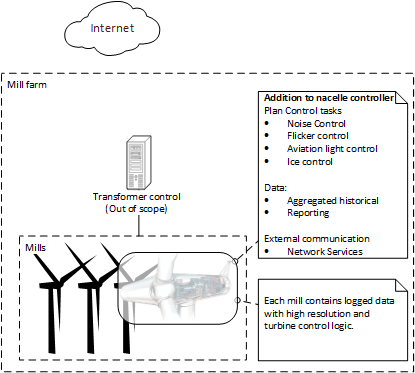
\includegraphics[width=0.7\textwidth,natwidth=610,natheight=642]{SystemOverviewsFuture.png} 
%	\captionsetup{format=plain,font=footnotesize,labelfont={bf,red},labelsep=quad,singlelinecheck=no}
%	\caption[Illustrates the future Siemens windmill farm setup]{
%		\label{fig:futureSiemensSetup} 
%		\footnotesize{%
%			This figure illustrates the future Siemens windmill farm setup.
%		}
%	}
%\end{figure}

\begin{figure}
	\centering
	\begin{sequencediagram} %Created using pgf-umlsd
		\newthread{reg}{:Park Regulartor}
		\newinst[2]{mill}{:Mill}
	
		\begin{sdblock}{each mill}{}
			\mess[1]{reg}{getCurrentStatus}{mill}
			\mess[1]{mill}{status}{reg}	
		\end{sdblock}
		
		\begin{call}{reg}{calculateAllSetpoints()}{reg}{}
		\end{call}
	
		\begin{sdblock}{each mill}{}
			\mess[1]{reg}{setNewSetpoint}{mill}
		\end{sdblock}
					
	\end{sequencediagram}

	\captionsetup{format=plain,font=footnotesize,labelfont={bf,red},labelsep=quad,singlelinecheck=no}
	\caption[Regulator calculation sequence]{
		\label{fig:dataComputationSequence} 
		\footnotesize{%
			Regulator calculation sequence.
		}
	}
\end{figure}

\subsection{Motivation}

Todays setup at Siemens Wind Power (\cref{sec:SiemensCase}) is an example of a system wished to be made less centralized. The current setup poses the following problems to Siemens:  

\begin{itemize} 
	\item Single point of failure. Should a WPS fail, a part of the windmill farm will become unavailable.
	\item Low scalability. The WPS's does not scale with the number of windmills.
	\item Low park regulation performance. Every windmill needs to return their current status to the Park Regulator, the set point for each windmill is calculated in the Park Regulator and finally the new set points can be pushed to the mills.
\end{itemize}

Siemens wishes to remove the WPS's by distributing their functionality to the windmills, utilizing the free capacity of the computers already residing in every windmill. This would increase redundancy and scalability and lower the possibility of a single point of failure. Furthermore, Siemens would like to look for ways to optimize the regulation sequence (see \cref{fig:dataComputationSequence}).




% Today windmills in windmill farm are connected to a single server that aggregates data, perform calculations, store data and handle communication with the outside world. These servers do not scale well with the size of the windmill farm, and they are a single point of failure. Therefor Siemens wishes to remove the servers by utilizing free capacity of the computers already residing in every windmill. 
%Currently there is some limited redundancy in data and availability but this could be greatly improved by distributing data and communication to the windmills. 
%Ease of access must be maintained even though computation and data is distributed. 
%This means routing traffic to a windmill with free capacity through  a single interface.

\section{Thesis aim}

The purpose of this thesis is to design, implement and evaluate a framework and associated tools for distributed computing systems development. The case from Siemens Windpower is an example of a production environment where the framework could be utilized. The goal is not to make a framework that is specific to the Siemens case but to make a general framework for the Siemens case and similar cases. 

The framework must be able to handle computation distributed on several nodes, communication between those nodes and distribution of data. This roughly leaves two essential components: A component that handles the virtual shared memory and a component that handles communication and distribution of tasks, with regards to the available resources on each node. Furthermore the framework must have a single interface for control of, and interaction with, all the nodes, in order to maintain the illusion of the windmill park serving as a single system. This means ease of access must be maintained even though computation and data is distributed among nodes. Traffic must be routed to a windmill with free capacity through a single interface, without external systems being aware of it.

The aim is to investigate and choose components, such that the best configuration is achieved with regards to distribution of data and computation across a production environment like the Siemens case. 

% % SKAL MÅSKE SÆTTES IND ???:
%To determine the best solution the different components will be weighed in terms of:
%\begin{itemize} 
%	\item Functionality. Does this component have the wanted functionality?
%	\item Scalability. Does this component scale well according to the Siemens case?
%	\item Redundancy. Doe
%	\item Performance. Does this component 
%\end{itemize}

The solution must work with the Siemens case, which presents the following constraints to the project:
\begin{itemize} 
	\item CPU power pr. node. Our solution must be able to run on a standard consumer x64 Intel CPU, since that is what each windmill are equipped with.
	\item Network bandwidth. Siemens told to assume close to unlimited bandwidth for the solution. 
\end{itemize}

Furthermore we aim to develop a prototype, which runs the developed framework, for proof of concept purposes. The framework will be compared to the existing Siemens solution with regards to availability and redundancy. 

%Distribution of computation tasks is the main research area and will be the focus of this thesis.




%\begin{itemize}
%	\item How do we distribute a database and computation across a production environment in the best possible way?
%	\item How do we define and measure performance?
%	\item Can it provide data redundancy and outperform current systems?
%	\item How many windmills are needed before it makes sense to makes sense to distribute the server?
%\end{itemize}
%
%We aim to investigate the possibility of making a framework and associated tools for developing a distributed system. 
%This framework must be able to handle computation distributed on several nodes, communication between those nodes and distribution of data. 
%The communication can be built on top of existing standards as for instance DDS. Data distribution can be built using existing systems like MongoDB. 
%Distribution of computation tasks is the main research area and will be the focus of this thesis.
%
%In order to achieve distributed computation on several nodes the framework must be able to perform load balancing and control the distribution of tasks on the nodes in the system. 
%Furthermore the framework must have a single interface for control of, and interaction with, all the nodes.  
%The goal is to create a test system, that can distribute and perform tasks but also to be able to plan ahead of time and know if there is available computation time.
%
%The case from Siemens Windpower is an example of a production environment where the framework could be utilized. 
%Our goal is not to make a framework that is only  specific for this case but to make a general framework for this and similar cases.

\section{Approach}

\section{Outline}
The remainder of this thesis is organized into the following chapters...

\section{Audience}
This thesis is aimed at an audience with a basic knowledge of...
